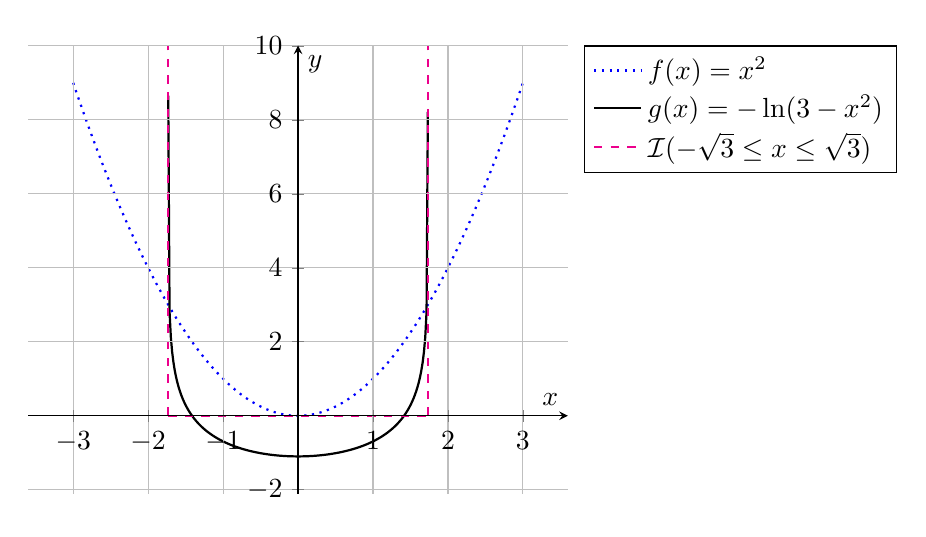
\begin{tikzpicture}
	\begin{axis}[
		axis lines = center,
		xlabel = {$x$},
		ylabel = {$y$},
		samples=200,
		domain=-3:3,  % Global domain setting for axis range
		legend pos=outer north east,
		grid = both,
		axis on top,
		enlargelimits = true,
		legend cell align={left},
		%title = {Comparison of $f(x)=x^2$ and $g(x)=-\ln(3 - x^2)$ with different domains}
		]
		
		% Plot f(x) = x^2 over the wider domain (-3, 3)
		\addplot[
		thick, dotted,
		blue,
		domain=-3:3,  % Wide domain for x^2
		]
		{x^2};
		\addlegendentry{$f(x) = x^2$}
		
		% Plot g(x) = -ln(3 - x^2) over the restricted domain (-1.73, 1.73)
		\addplot[
		thick,
		black,
		domain=-1.73199999:1.7319999,  % Restricted domain for -ln(3 - x^2)
		]
		{-ln(3 - x^2)};
		\addlegendentry{$g(x) = -\ln(3 - x^2)$}
		
		\addplot[domain=-1.73199999:1.7319999, samples=3, thick, magenta, dashed] {0};
		\addlegendentry{$\mathcal{I}(-\sqrt{3}\leq x \leq \sqrt{3}$)}
		% Indicate the "infinity" outside [-3, 3] with vertical asymptotes
		\draw[dashed, thick, magenta] (axis cs:-1.73199999,0) -- (axis cs:-1.73199999,10);  % Vertical asymptote at x = -3
		\draw[dashed, thick, magenta] (axis cs:1.73199999,0) -- (axis cs:1.73199999,10);    % Vertical asymptote at x = 3
		
		% Label the "infinity" on the graph
		\node at (axis cs:-1.73199999, 10) [above] {$\infty$};
		\node at (axis cs:1.73199999, 10) [above] {$\infty$};
		
		
	\end{axis}
\end{tikzpicture}